\documentclass[letterpaper,12pt]{article}
\usepackage[margin=.5in]{geometry}
\usepackage{graphicx}  % Include figure files
\usepackage{xcolor}  % Allow for a color text
\usepackage{amsmath}  % math fonts
\usepackage{amsfonts}  % math fonts
\usepackage{latexsym}  % math fonts
\usepackage{amssymb}  % math fonts
\usepackage{mathtools} % Give more control of how equations are displayed
\usepackage{appendix} % Lets you create an appendix
\usepackage[numbered]{matlab-prettifier} % Let's me import MATLAB code in a nice format
\usepackage{indentfirst} % This indents the first paragraph. By default latex won't do it.

%\setlength{\parskip}{1em} % This skips a line when making new paragraphs
\newtagform{show_eq}{(Eq.\ }{)}  % how the equation numbers are displayed
\usetagform{show_eq} % this goes with the \newtagform

\begin{document}

% ================================== Title Page ==========================================
\begin{titlepage}
 \begin{center}
 \vspace*{1in}
{\Huge Simulation of a Rotor with Gear Train Driving a Propeller}\\
    \bigskip
    by\\
    \bigskip
    {\Large Kevin Moran} \\
    \bigskip
    Date : November 1st, 2020

    \bigskip\bigskip\bigskip
    University of Southern California\\
    Aerospace and Mechanical Engineering Department\\
    AME 302 : System Dynamics
 \end{center}
\end{titlepage}

% ================================== Main Text =====================================

% --------------------------------- Impulse Images ------------------------------
\section{Transfer Function Analysis}
The transfer function for the angular velocity of the propeller, $\omega_p$, can be written as
\begin{equation}
    \frac{\Omega (s)}{T (s)} = \frac{Ncs + Nk}{s^3\sigma_3 + s^2\sigma_2 + s\sigma_1 + \sigma_0}
\end{equation}

where

\begin{align*}
        N &= N_1N_2\\
        \sigma_3 &= NJ_RJ_p \\
        \sigma_2 &= J_pc + J_pN^2b_1 + J_rN^2b_2 + J_rN^2c\\
        \sigma_1 &= J_pk + b_2c + J_rN^2k + N^2b_1b_2 + N^2b_1c\\
        \sigma_0 &= N^2b_1k + b_2k
\end{align*}
and the variables $J_r,\ J_p,\ b_1,\ b_2,\ c,\ k,\ N_1,\ and \ N_2$ are system parameters. During this simulation, the stiffness coefficient of the flexible rod, $k$, was changed during each iteration, ranging from 5 to 1000 (non-dimensional values). 

\subsection{Stability, Frequency, and Lower Order Approximation}
During each iteration, the poles of the transfer function were determined using the MATLAB Control System Toolbox and it was found that varying the stiffness coefficient had little affect on the real components of the poles. In each case, all of the real components satisfied the stability requirements and demonstrated the requirement for the existence of a steady state (i.e., $Re[p_i] < 0$). Furthermore, comparing the real components of the polls shows that the system can be approximated as a 2nd order system. Regardless of the stiffness coefficient, the real components of the poll were estimated to be -.00173 (multiplicity of 2) and -.0128.

The imaginary component, however, significantly changed during each iteration. The magnitude of the imaginary component of the poles increased along with the stiffness coefficient. Furthermore, since the damped frequency of a system is related to the imaginary component of the poles, it was also anticipated that the frequency of oscillation for the propeller to also increase. 


\subsection{Impulse Function Steady State}
By using the final value theorem, we can determine the steady state for the impulse input as,
\begin{equation}
    \omega (t_{ss}) = \lim_{s\to 0} s\Omega(s) = \lim_{s\to 0} \frac{400(N c s^2+N k s)}{s^3\sigma_3 + s^2\sigma_2 + s\sigma_1 + \sigma_0} = 0
\end{equation}
which also supports the notion that a damped system starting with a finite amount of energy eventually returns to rest.

\subsection{Step Function Steady State}
Once again, applying the final value theorem to the system with a step function input yields
\begin{equation}
    \omega (t_{ss}) = \lim_{s\to 0} s\Omega(s) = \lim_{s\to 0} \frac{400(Ncs+Nk)}{s^3\sigma_3 + s^2\sigma_2 + s\sigma_1 + \sigma_0} = \frac{400N}{N^2b_1 + b_2} \approx 189
\end{equation}
After applying the limit, it can be shown that the parameter $k$ cancels out in the numerator and denominator.   

\section{Simulation Results}
The following pages contain graphs that represent the results from the simulation. Graphs are primarily grouped by stiffness coefficients and illustrate the results through the entire time domain. Additionally, two subplots illustrate time domains of interest.

In each case, the impulse and step responses of the system agreed with the results of the final value theorem. Furthermore, as the stiffness coefficient increases, the frequency of the oscillations also increase and support the anticipated results from the transfer function poles.

\begin{table}[h]
    \centering
    \begin{tabular}{c|c|c|c|c|c|c}
         k & $f_{impl}$ [Hz] & $f_{step}$ [Hz] & $Imp\ A_{t0 : t20}$ & $Imp\ A_{t1980 : t2000}$ & $Step\ A_{t460 : t480}$ & $Step\ A_{t1480 : t1500}$ \\
         \hline
         5 & 0407 & .0408 & - & - & - & - \\
         15 & .0706 & .0707 & 7.05 & .171 & 4.95 & .892\\
         50 & .129 & .129 & 4.75 & .171 & 2.71 & .49 \\
         100 & .182 & .182 & 4.76 & .171 & 1.92 & .346\\
         500 & .407 & .408 & 4.78 & .171 & .85 & .154\\
         1000 & .576 & .576 & 4.76 & .170 & .605 & .109
    \end{tabular}
    \caption{Oscillation frequency for impulse and step responses. Frequency was determined by taking the time difference between local maximas and taking the inverse of the average time difference. The subscripts denotes the time intervals and any entry with a dash indicated that there wasn't enough data to make accurate calculations. }
\end{table}



\begin{figure}[ht]
    \centering
    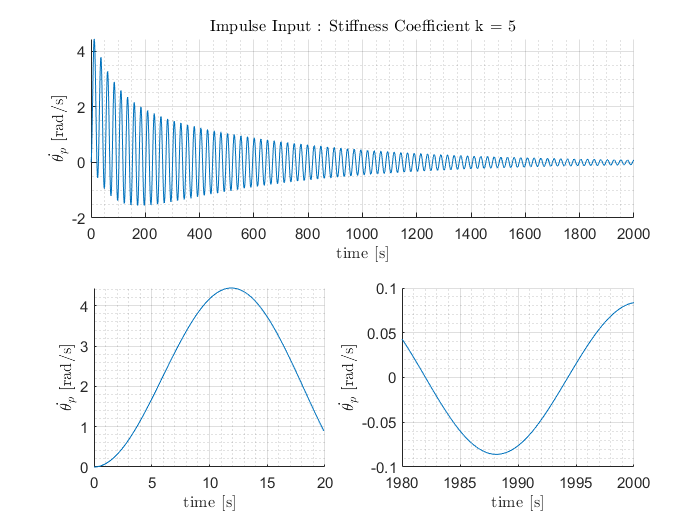
\includegraphics[scale = .8]{Images/Impulse_k5.png}
    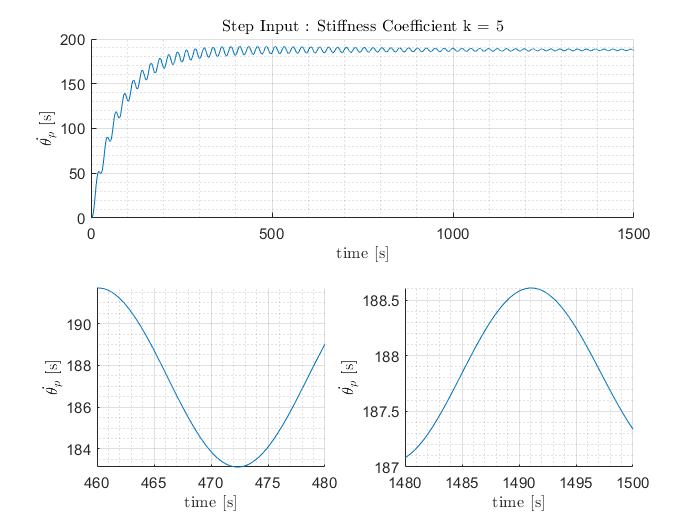
\includegraphics[scale = .8]{Images/StepInput_k5.png}
\end{figure}

\begin{figure}[ht]
    \centering
    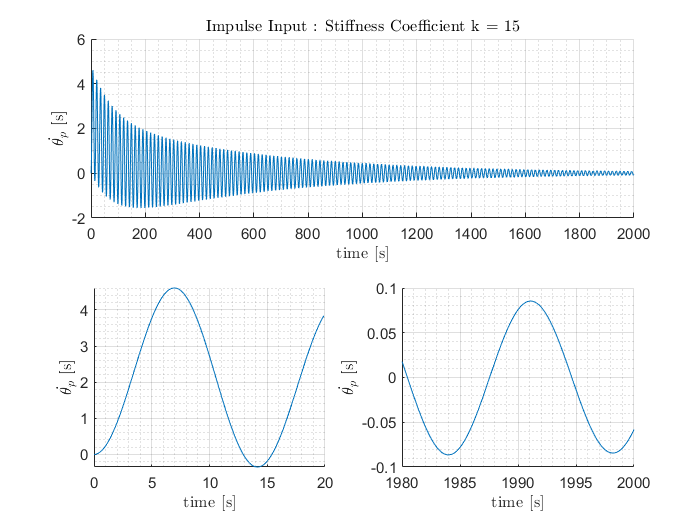
\includegraphics[scale = .8]{Images/Impulse_k15.png}
    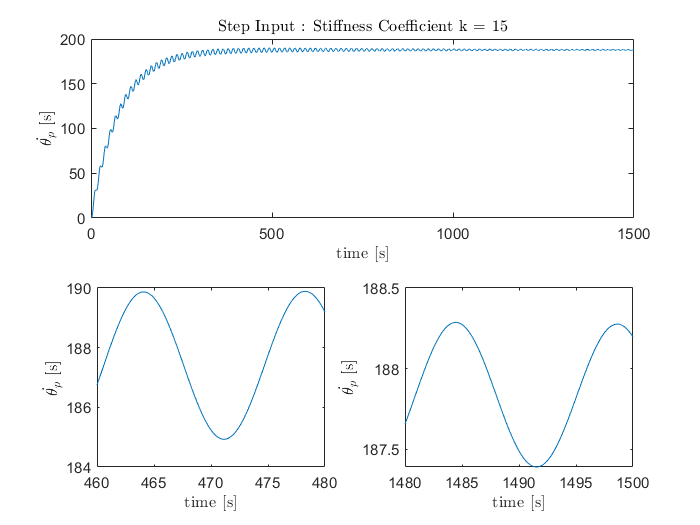
\includegraphics[scale = .8]{Images/StepInput_k15.png}
\end{figure}

\begin{figure}[ht]
    \centering
    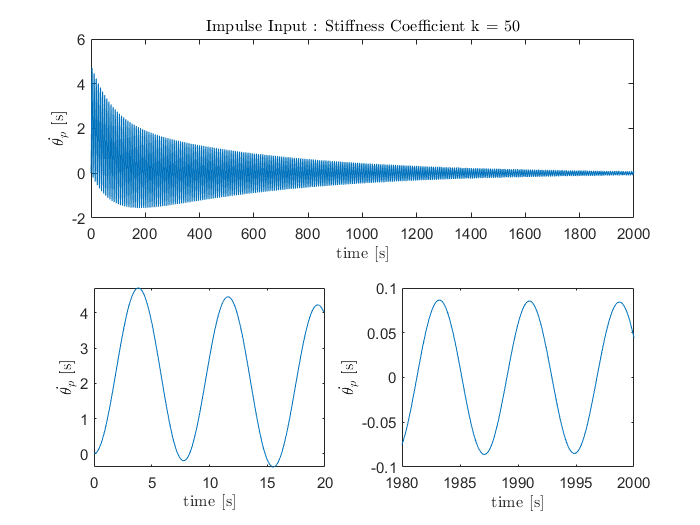
\includegraphics[scale = .8]{Images/Impulse_k50.png}
    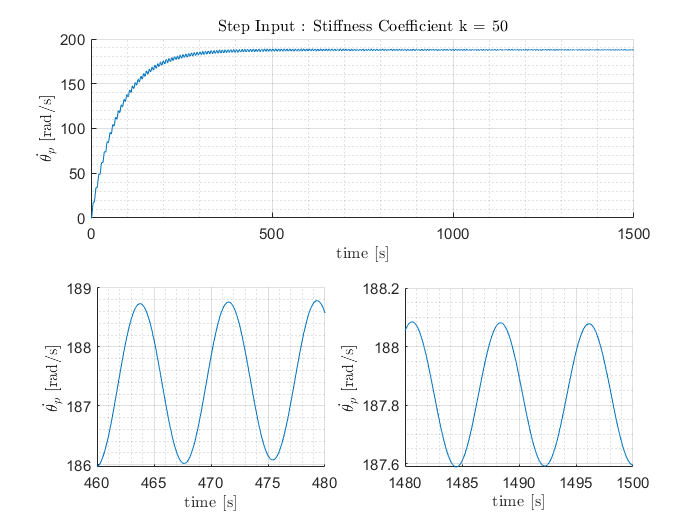
\includegraphics[scale = .8]{Images/StepInput_k50.png}
\end{figure}

\begin{figure}[ht]
    \centering
    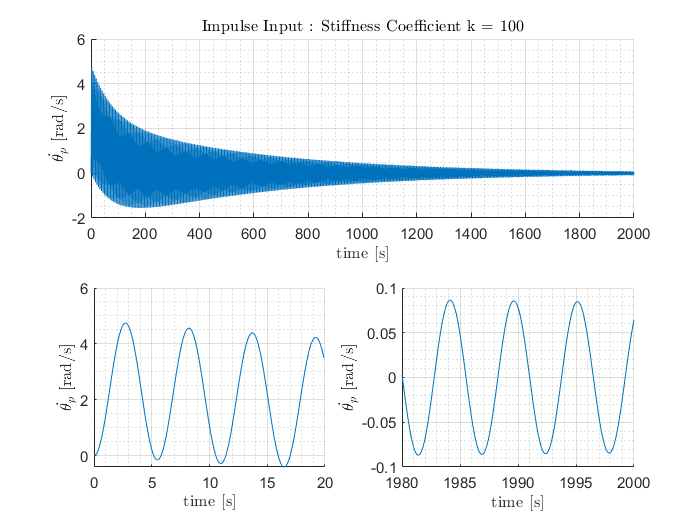
\includegraphics[scale = .8]{Images/Impulse_k100.png}
    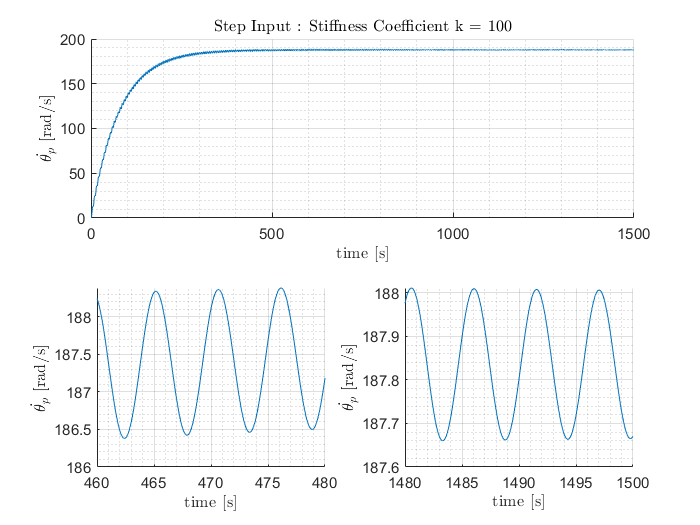
\includegraphics[scale = .8]{Images/StepInput_k100.png}
\end{figure}

\begin{figure}[ht]
    \centering
    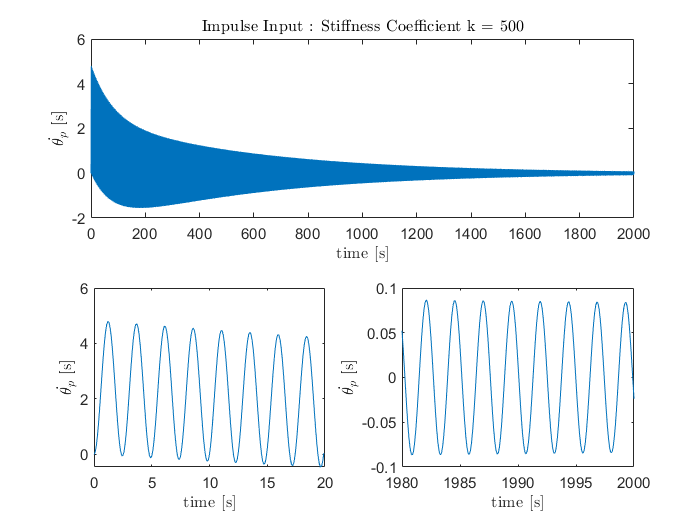
\includegraphics[scale = .8]{Images/Impulse_k500.png}
    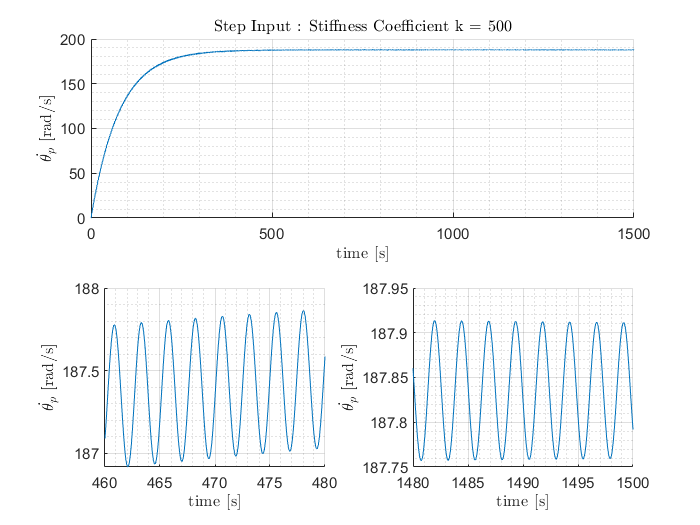
\includegraphics[scale = .8]{Images/StepInput_k500.png}
\end{figure}

\begin{figure}[ht]
    \centering
    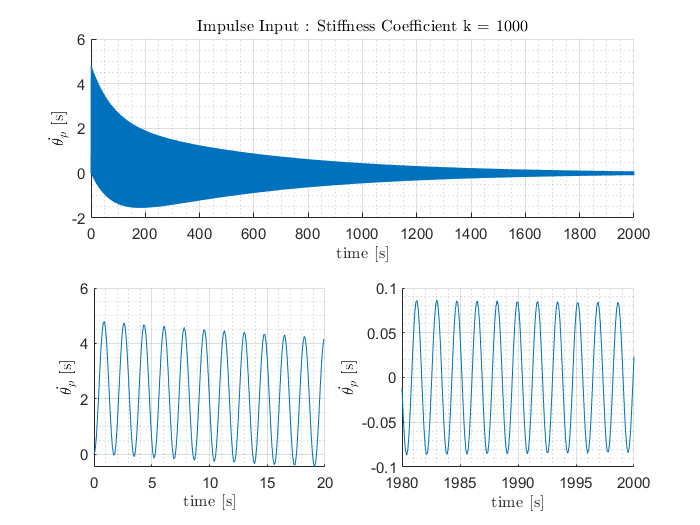
\includegraphics[scale = .8]{Images/Impulse_k1000.png}
    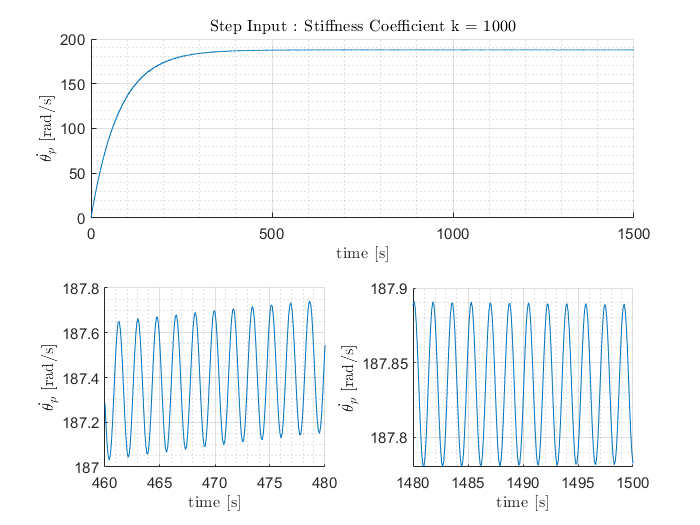
\includegraphics[scale = .8]{Images/StepInput_k1000.png}
\end{figure}

\end{document}